\documentclass[12pt]{article}

\usepackage{mathtools} % Mathematical tools to use with amsmath
\usepackage{amsfonts} % TeX fonts from the American Mathematical Society
\usepackage{ifxetex}
\usepackage{indentfirst} % Indent first paragraph after section header
\ifxetex
  \usepackage{mathspec} % Specify arbitrary fonts for mathematics in XeTeX
  \usepackage{fontspec} % Advanced font selection in XeLaTeX and LuaLaTeX
  \usepackage{polyglossia} % Multilingual support for XeLaTeX
\else
  \usepackage[T1,T2A]{fontenc}
  \usepackage[utf8x]{inputenc}
  \usepackage[ukrainian]{babel}
\fi

\usepackage{ifxetex}
\ifxetex
  % mathspec
  \setmathsfont(Digits,Latin,Greek){Times New Roman}

  % fontspec
  \defaultfontfeatures{Mapping=tex-text}
  \setmainfont{Times New Roman}
  \setmonofont[Mapping=tex-text]{Fantasque Sans Mono}
  \newfontfamily\cyrillicfont{Times New Roman}
  \newfontfamily\cyrillicfontsf[Script=Cyrillic]{Fantasque Sans Mono}
  \newfontfamily\cyrillicfonttt[Script=Cyrillic]{Fantasque Sans Mono}

  % polyglossia
  \setdefaultlanguage{ukrainian}
\fi

%поля
\usepackage{vmargin}
\setpapersize[portrait]{A4}
\setmarginsrb{25mm}{10mm}{10mm}{25mm}{5mm}{3mm}{0mm}{0mm}
%\usepackage[left=25mm,right=15mm,
%    top=12mm,bottom=12mm,bindingoffset=0cm, footskip=7mm]{geometry}

%параметри
\parindent=1cm  %установка оступа абзаца
\usepackage{indentfirst} %абзацный отступ в начале раздела 
\pagestyle{plain} % нумерация страниц вкл.
\linespread{1.5} %межстрочный интервал

%верхний колонтилут
\usepackage{fancyhdr} % пакет для установки колонтитулов
\pagestyle{fancy} % смена стиля оформления страниц
\fancyhf{} % очистка текущих значений
\fancyhead[R]{\thepage} % установка верхнего колонтитула
\renewcommand{\headrulewidth}{0pt} % убрать разделительную линию

%форматування заголовків
\usepackage{titlesec}
\titleformat{\section}[block]{\normalfont\large\centering\bfseries}{\thesection}{1ex}{}
\titleformat{\subsection}[block]{\normalfont\normalsize\centering\bfseries}{\thesection}{1ex}{}

\usepackage{graphicx}  %изображения
\graphicspath{{pic/}}
\DeclareGraphicsExtensions{.pdf,.png,.jpg}
\usepackage{caption}

% \usepackage{xcolor} %колір посилань
\usepackage[
  colorlinks=true, allcolors=black,
]{hyperref} % для посилань
% \definecolor{linkcolor}{HTML}{799B03} % цвет ссылок
% \definecolor{urlcolor}{HTML}{799B03} % цвет гиперссылок
% \hypersetup{pdfstartview=FitH,  linkcolor=linkcolor,urlcolor=urlcolor, colorlinks=true}

\usepackage{color} %% это для отображения цвета в коде
\usepackage{xcolor}
\usepackage{listings} %% собственно, это и есть пакет listings

\usepackage{caption}
\DeclareCaptionFont{white}{\color{white}} %% это сделает текст заголовка белым
%% код ниже нарисует серую рамочку вокруг заголовка кода.
\DeclareCaptionFormat{listing}{\colorbox{gray}{\parbox{\textwidth}{#1#2#3}}}
\captionsetup[lstlisting]{format=listing,labelfont=white,textfont=white}

% listed
\usepackage{listings} % Typeset source code listings using LaTeX
\lstset{language=Python,
  basicstyle=\ttfamily,
  keywordstyle=\color{blue}\ttfamily,
  stringstyle=\color{red}\ttfamily,
  commentstyle=\color{green}\ttfamily,
  morecomment=[l][\color{magenta}]{\#}
}

\usepackage{minted}
\newminted{python}{baselinestretch=1.2,fontsize=\footnotesize,linenos,breaklines}
\newmintinline{python}{showspaces}

\numberwithin{equation}{section}
\numberwithin{figure}{section}

\usepackage{titlesec} % Select alternative section titles
\titleformat{\section}
  {\newpage\normalfont\Large\bfseries\centering}{\thesection. }{0pt}{}
\titleformat{\subsection}
  {\normalfont\large\bfseries\centering}{\thesubsection. }{0pt}{}
\titleformat{\subsubsection}
  {\normalfont\large\bfseries\centering}{\thesubsubsection. }{0pt}{}

\usepackage[section]{placeins}

\begin{document}
%титульный лист	
		\begin{center}
		\hfill \break
		\large{МІНІСТЕРСТВО ОСВІТИ ТА НАУКИ УКРАЇНИ} \\
		\large{ДНІПРОВСЬКИЙ НАЦІОНАЛЬНИЙ УНІВЕРСІТЕТ ІМ. О. ГОНЧАРА} \\
		\large{ФАКУЛЬТЕТ ПРИКЛАДНОЇ МАТЕМАТИКИ} \\
		\large{КАФЕДРА КОМП'ЮТЕРНИХ ТЕХНОЛОГІЙ} \\
		\hfill\break
		\hfill\break
		\hfill\break
		\hfill\break
		\large{\bfseries ЛАБОРАТОРНА РОБОТА} \\
		\normalsize{з дисципліни: Моделювання складних систем} \\
		\normalsize{на тему: <<Побудова математичної моделі гідроелектростанції>>} \\
		\end{center}
		
		\hfill\break
		\hfill\break
		\hfill\break
		\begin{flushright}
		\begin{tabular}{l}
		\underline{Виконали:} \\
		студенти групи ПК-21м-1 \\
		Панасенко Є. С. \\
		Гриценко А. О. \\
		Доценко Т.С.\\
		Ємельянова Ю. С. \\
		Олійник Д. І. \\
		Яцевська О. О. \\
		\end{tabular}
		\end{flushright}
		\hfill\break
		\hfill\break		
		\hfill\break
		\hfill\break
		\begin{center}
		м.Дніпро, 2021
		\end{center}	
        
\thispagestyle{empty}
	
\tableofcontents
	
\section{Постановка задачі}

\begin{enumerate}
	\item Провести огляд джерел предметної області та розглянути існуючі підходи до побудови математично моделі гідроелектростанції.
	\item Побудувати математичну модель гідроелектростанції, використовуючи підхід на основі балансових співвідношень.
	\item Розробити програмне забезпечення на основі побудованої математичної моделі та знайти наближений розв’язок задачі.
	\item Провести дослідження отриманого розв’язку математичної моделі при різних значеннях параметрів системи.
	\item Сформулювати висновки.  
\end{enumerate}

\newpage

\section{Принцип роботи гідроэлектростанції}

\subsection{Водна енергія у природі}

Під впливом сонячного випромінювання з поверхні океанів, морів, материків випаровується вода. Повітряні потоки розносять водяні пари над земною поверхнею. Коли водні пари конденсуються в верхніх холодних шарах атмосфери, вони опадають на землю у вигляді дощу та снігу. Під впливом сили тяжіння частки води переміщуються по поверхні землі на найбільш низькі рівні. Таким чином утворюються річки та струмки, які вливаються у моря та океани. 

Коли під впливом сонячного випромінювання чистки води випаровуються, вони знову піднімаються у верхні шари атмосфери, виконуючі нескінчений колообіг води у природі, що складає одну з основ життя на Землі.

Вода  має механічну енергію і, пересуваючись руслом, поступово втрачає свою потенційну енергію. Деяка її частка переходить у кінетичну, швидкісну енергію рухомих мас. Проте більша частка витрачається на роботу з подолання сил тертя між частками води, між водяним потоком та руслом, розмиваючи його та переміщуючи наноси. В кінцевому рахунку енергія перетворюється в теплову та розсіюється. Однак механічна енергія води, або гідравлічна, неперервно поновлюється.

Створивши на ріках штучні гідротехнічні споруди та встановивши необхідне обладнання, можна використовувати частку гідравлічної енергії для потреб людства.

Проблеми використання енергії води вивчає гідроенергетика, яка є однією з складових галузі, що називається електроенергетикою. 

\subsection{Енергія та міць водяного потоку. Гідроенергетичні ресурси}\label{sec:task}

Припустимо, що потік має постійні по довжині русла перетин та швидкість течії води, при цьому бічна приточність відсутня. Для визначення енергії водяного потоку розглянемо проміжок АВ. Скористуємося рівнянням Бернуллі, яке визначає реальну енергію потоку, тобто енергію маси води, вага якої дорівнює 1 Н (одному ньютону): 

\begin{equation}\label{eq:1}
e = z + \dfrac{p}{pg} + a \dfrac{v^2}{2g},
\end{equation}

Де $e$ - питома енергія (Дж або Н $\cdot$ м); $z$ - геометрична висота точки перетину над рівнем моря або над довільною площиною порівняння (00, м); $p$ - тиск в точці перетину потоку (Па); $v$ - середня швидкість течії води (м/с); $\rho$ - щільність води (кг/м$^3$); $g=9.81$ м/с$^2$ - прискорення вільного падіння; $a=1.03 / 1.1$ - безрозмірний коефіцієнт Коріоліса, що враховує неровномірність розподілу швидкостей по перетину.

Сума $a+z / (pg)=h$ визначає запас питомої потенційної енергії у даному перетині, тобто запас енергії висотного положення $z$ та енергії тиску $p/(pg)$. Для всіх точок перетину потоку із вільною поверхнею сумарна потенційна енергія $h$ постійна, оскільки зі збільшенням $z$ на таке саме значення зменшується $p/(pg)$. Питома потенційна енергія у перетені потока можна визначати висотою відмітки вільної поверхні над площиною порівняння. Для перетенів А та В ця енергія відповідно дорівнює:

\begin{equation}\label{eq:2}
\left\{
\begin{array}{l}
    h_A = \nabla A; \\
    h_B = \nabla B.
\end{array}
\right.
\end{equation}

Доданок $a\dfrac{v^2}{2g}$ визначає питому кінетичну (швидкісну) енергію. Рівняння \ref{eq:1} характеризує запас всієї питомої енергії $e$ в даному перетині. Згідно до закону збереження енергії в потоці рідини енергія $e_{AB}$, що виділяється під час руху на проміжку АВ, дорівнює різниці енергії потоку в перетинах А та В:
\begin{equation}\label{eq:3}
e_{AB} = e_A - e_B
\end{equation}

Якщо прийняти $v_A = v_B$, різницею кінетичних енергій можна знехтувати:
\[
\left(
a\frac{v^2_A}{2g} - a\frac{v^2_B}{2g} = 0
\right)
\]

Тоді енергія водяного потоку на проміжку АВ складатиме:
\begin{equation}\label{eq:4}
e_{AB} = h_A - h_B = \nabla A - \nabla B = H_{AB}
\end{equation}

де $H_{AB}$ - перепад рівней вільної поверхні на проміжку АВ. При визначені повної енергії потоку необхідно врахувати водність потоку, що обраховується витратою води $Q$ (м$^3$/с). Припустимо, що протягом часу $t$ через проміжок АВ проходить об'єм води $Qt$ (м$^3$), вага якого складає $Qt\rho g$. Тоді повна енергія (Дж) що виділилася на проміжку:

\begin{equation}\label{eq:5}
Е_{AB} = H_{AB} Qt\rho g
\end{equation}

Визначимо міць потоку $N_{AB}$, тобто енергію, що виділається за 1с:

\begin{equation}\label{eq:6}
N_{AB}=E_{AB}|t = H_{AB}Q\rho g.
\end{equation}

В (1.6) розмірність $N_{AB}$ буде:

\[
\text{м}\frac{\text{м}^3}{\text{c}}\frac{\text{H}}{\text{м}^3} = \frac{\text{H}\cdot \text{м}}{\text{с}} = \frac{\text{Дж}}{\text{с}} = \text{Вт}.
\]

Ват достатньо мала одиниця вимірювання, тому в енергетиці використовують більш великі одиниці - кіловат (1кВт = 1000Вт) та мегавати (1МВт = 1000кВт=10$^6$). Якщо представити $N_{AB}$ у кіловатах та прийняти чисельні значення прискорення вільного падіння $g=9.81$ м$^2$/с та щільність $\rho = 1000$ кг/м$^3$, отримаємо:

\begin{equation}\label{eq:7}
N_{AB}=9.81QH_{AB}
\end{equation}

Кількість електроенергії у промисловості прийнято вимірювати у кіловат-годинах (1кВт$\cdot$г = $3.6\cdot 10^6$ Дж). Якщо вимірювати час $T$ у годинах, то енергія $E_{AB}$ (кВт$\cdot$г) буде:
$$
E_{AB} = 9.81QH_{AB}T,
$$

зокрема енергія, що виділилась за рік, T=8760г.

\subsection{Принцип роботи гідроелектростанції}

 Сьогодні сучасні гідроелектростанції – це величезні споруди на гігават встановленої потужності. Однак принцип роботи будь-якої ГЕС залишається в цілому досить простим і всюди майже повністю однаковим. Напір води, спрямований на лопаті гідротурбіни, призводить її в обертання, а гідротурбіна в свою чергу, будучи з’єднана з генератором, обертає генератор. Генератор виробляє електроенергію, яка і подається на трансформаторну станцію, а потім і на ЛЕП.
 
 У машинному залі гідроелектростанції встановлені гідроагрегати, які перетворюють енергію потоку води в енергію електричну, а безпосередньо в будівлі гідроелектростанції розташовуються всі необхідні розподільні пристрої, а також пристрої управління і контролю роботи ГЕС.

Потужність гідроелектростанції залежить від кількості і від напору води, що проходить через турбіни. Безпосередньо натиск виходить завдяки направленого руху потоку води. Це може бути вода накопичена у греблі, коли в певному місці на річці будується гребля, або ж натиск виходить завдяки деривації потоку, – це коли вода відводиться від русла по спеціальному тунелю або каналу.

Так, гідроелектростанції бувають греблі, дериваційними і гребле-дериваційними. Найбільш поширені греблі ГЕС мають в своїй основі греблю, перегороджує русло річки. За греблею вода піднімається, накопичується, створюючи свого роду водяний стовп, що забезпечує тиск і натиск. Чим вище гребля – тим сильніше натиск. Найвища в світі гребля має висоту 305 метрів, це гребля на Цзіньпінской ГЕС потужністю 3,6 ГВт, що на річці Ялунцзян в західній частині провінції Сичуань на Південно-Западній території Китаю.

Гідростанції, що використовують енергію води, бувають двох типів. Якщо річка має невелике падіння, але щодо багатоводна, то за допомогою греблі, що перегороджує річку, створюють достатню різницю рівнів води.

Над греблею утворюється водосховище, що забезпечує рівномірну роботу станції протягом року. Біля берега нижче греблі, в безпосередній близькості до неї встановлюється водяна турбіна, поєднана з електричним генератором (пригребельного станція). Якщо річка судноплавна, то біля протилежного берега робиться шлюз для пропуску судів.Якщо ж річка не дуже багатоводна, але має велике падіння і бурхливу течію (наприклад, гірські річки), то частина води відводиться по спеціальному каналу, має набагато менший ухил, ніж річка. Канал цей іноді має протяжність в кілька кілометрів. Іноді умови місцевості змушують замінити канал тунелем (для потужних станцій). Таким чином створюється значна різниця рівнів між вихідним отвором каналу і нижньою течією річки. У кінця каналу вода надходить в трубу з крутим нахилом, у нижнього кінця якої розташовується гідротурбіна з генератором. Завдяки значній різниці рівнів вода набуває велику кінетичну енергію, достатню для живлення станції (дериваційні станції). Подібні станції можуть мати більшу потужність і ставитися до розряду районних електростанцій. На найменших станціях турбіна іноді замінюється менш ефективним, за дешевшими водяним колесом.


\subsection{Сучасна ситуація гідроенергетики в Україні}

На сучасному етапі гідроенергетичні об’єкти займають вагоме місце у загальній енергосистемі України. Гідроенергетика має низку суттєвих переваг як порівняно з традиційними методами виробництва енергії, а саме:

\begin{itemize}
	\item генерація без використання викопного органічного та ядерного палива;
	\item низька собівартість виробітку електроенергії;
	\item запобігання паводкам;
	\item значний термін служби та висока надійність експлуатації;
	\item додаткові можливості для ведення рибного господарства, зрошення, водопостачання;
	\item можливість оперативного регулювання потужності. 
\end{itemize}

Гідроенергетика – єдина «зелена» галузь енергетики, що може зібрати надлишок енергії та зберегти його до того моменту, коли в мережі буде дефіцит. Крім того, гідроелектростанції, на відміну від сонце- та вітро-, не залежать від погодних умов і можуть генерувати електроенергію в будь-який час, що робить їх надзвичайно цінним джерелом балансуючих потужностей для Об’єднаної енергосистеми.

\begin{figure}[!htb]
	\centering
	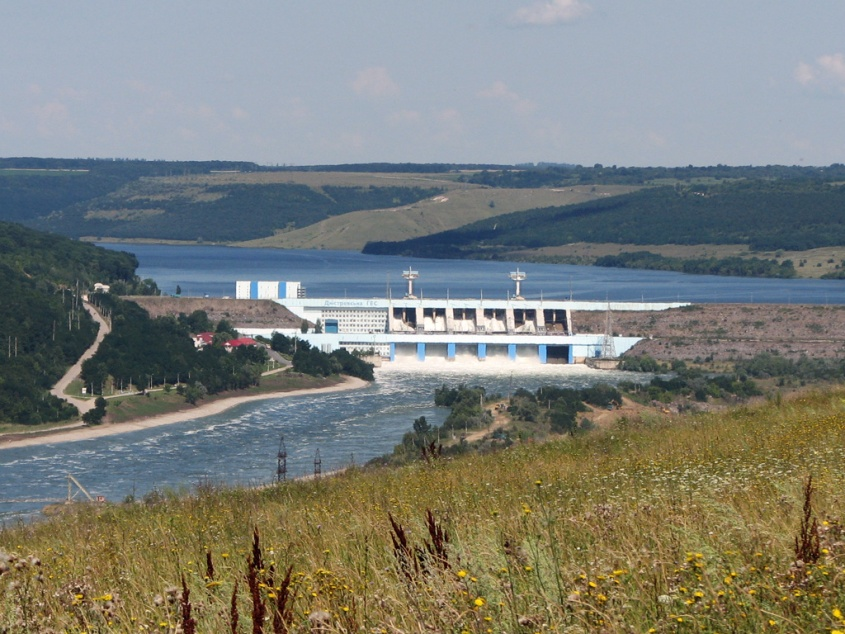
\includegraphics[width=0.7\linewidth]{03.PNG}
	\caption{Дністровська ГАЕС}
\end{figure}

На сьогодні, існуюча потужність великих ГЕС становить біля 9\% відсотка всіх генеруючих потужностей ОЕС України, однак існує потенціал для подальшого зростання до 15-20\%. Окремим напрямом розвитку гідроенергетики в Україні є розвиток малої гідроенергетики на існуючих водоймищах, магістральних каналах, а також реконструкція об'єктів малої гідроенергетики, що виконують функцію із захисту прилеглих територій від повеней.
ГЕС та ГАЕС зайняли 4-е місце в обсязі генерації у 2020р, виробивши 5,1\% (з них ГЕС - 4\%, ГАЕС -1\%), або 7,58 млрд кВт-год, що на 3,7\% менше показника генерації у 2019р (7,86 млрд кВт-год). При цьому споживання ГАЕС у насосному режимі (споживання електроенергії станціями, для балансування енергосистеми) збільшилось на 16,3\% - до 2,13 млрд кВт-год.
Пріоритетом розвитку гідроенергетики України відповідно до оновленої редакції Енергетичної стратегії України на період до 2030 року визначено будівництво додаткових гідро- і гідроакумулюючих потужностей. Поряд із пріоритетними напрямами використання потенціалу великої гідроенергетики, існує можливість використання потенціалу малих рік України.
Наразі на території України експлуатується майже 50 малих ГЕС. У таблиці нижче приведені деякі із діючих ГЕС та ГАЕС:

\noindent\begin{tabular}{|c|c|c|p{2cm}|p{2cm}|}
\hline
Назви & Ріки & Розташування & Фактична\linebreak потужність,\linebreak МВт & Побудова\linebreak першої\linebreak черги \\
\hline
Дніпровська ГЕС	& Дніпро & Запоріжжя & 1569 & 1927-1932 \\
Середньодніпровська ГЕС	& Дніпро & Кам'янське	& 352	& 1963 \\
Дністровська ГАЕС	& Дністер	& Розкопинці	& 972	& 1983-2015 \\
Дністровська ГЕС-1	& Дністер	& Новодністровськ	& 702	& 1973-1981 \\
Дністровська ГЕС-2	& Дністер	& Нагоряни & 40,8	& 1982-2000 \\
Канівська ГЕС	& Дніпро	& Канів	& 444	& 1972 \\
Каховська ГЕС	& Дніпро	& Нова Каховка	& 351	& 1955 \\
Київська ГАЕС	& Дніпро	& Нові Петрівці	& 235,5	& 1970 \\
Київська ГЕС	& Дніпро	& Вишгород	& 408,5	& 1964 \\
Кременчуцька ГЕС	& Дніпро	& Світловодськ	& 692	& 1959 \\
Ташлицька ГАЕС	& Південний Буг	& Южноукраїнськ	& 302	& 1981-2007 \\
Теребле-Ріцька ГЕС	& Теребля та Ріка	& Хустський район	& 27	& 1949-1956 \\
\hline

\end{tabular}
\newpage
	
\section{Побудова математичної моделі гідроэлектростанції}
Введемо змінні та константи системи:
\begin{itemize}
\item $t$ - момент часу у секундах,
\item $E(t)$ - кількість енергії, яка може бути вироблена за допомогою гідроелектростанції у момент часу $t$,
\item $P(t)$ - швидкість зміни кількості виробляємої енергії, тобто $P(t)=E'(t)$,
\item $E_{AB}$ - кількість енергії, яка може бути вироблена завдяки греблі за час $T$,
\item $H_{AB}$ - перепад висот, утвореної за допомогою греблі,
\item $Q$ - об'єм води який проходить за секунду у турбіні,
\item $T$ - деякий проміжок часу у секундах,
\item $g$ - прискорення вільного падіння.
\end{itemize}

З розділу \ref{sec:task} відомо, що:
\[E_{AB}=gQH_{AB}T\]

Таким чином можна визначити, що за час $dt$, енергія зміниться на $dE$, таким чином отримаємо:
\[dE = gQH_{AB}dt\]

Звідси отримаємо диференціальне рівняння:
\[\cfrac{dE}{dT} = gQH_{AB}\]
або
\[E' = gQH_{AB}\]

Таким чином можна визначити яка кількість енергії може бути вироблена у момент часу, за допомогою гідроэлектростанції. Нехай у початковий момент часу не енергія дорівнює 0:
\[E(0)=0\]

Отримаємо систему:
\[\left\{
\begin{array}{l}
E' = gQH_{AB}\\E(0)=0
\end{array}
\right.\]

Цю систему можна вирішити за допомогою методу Эйлера, поділимо проміжок часу на шаг $h$ рівний одній неділі, тобто $h=604800$, отримаємо систему:
\[\left\{
\begin{array}{l}
E[i+1] = E[i] + hf(t)\\
P[i+1] = f(t)
\end{array}
\right.\]

\[\left\{
\begin{array}{l}
E[i+1] = E[i] + hgQH_{AB}\\
P[i+1] = gQH_{AB}
\end{array}
\right.\]

Візьмемо для розгляду ДніпроГЕС, ця гідроелектростанція завдяки греблі утворює перепад висот у 50 метрів. Наведемо показання витрат води через турбіни за два роки:\\

\begin{tabular}{|c|c||c|c||c|c||c|c|}\hline
Дата & Показ. & Дата & Показ. & Дата & Показ. \\
& $\text{м}^3/\text{c}$ && $\text{м}^3/\text{c}$ && $\text{м}^3/\text{c}$ \\\hline
2019-01-01 & 793 & 2019-08-13 & 793 & 2020-03-24 & 793 \\\hline
2019-01-08 & 678 & 2019-08-20 & 678 & 2020-03-31 & 678 \\\hline
2019-01-15 & 517 & 2019-08-27 & 517 & 2020-04-07 & 517 \\\hline
2019-01-22 & 947 & 2019-09-03 & 947 & 2020-04-14 & 947 \\\hline
2019-01-29 & 882 & 2019-09-10 & 882 & 2020-04-21 & 882 \\\hline
2019-02-05 & 948 & 2019-09-17 & 948 & 2020-04-28 & 948 \\\hline
2019-02-12 & 877 & 2019-09-24 & 877 & 2020-05-05 & 877 \\\hline
2019-02-19 & 939 & 2019-10-01 & 939 & 2020-05-12 & 939 \\\hline
2019-02-26 & 916 & 2019-10-08 & 916 & 2020-05-19 & 916 \\\hline
2019-03-05 & 965 & 2019-10-15 & 965 & 2020-05-26 & 965 \\\hline
2019-03-12 & 772 & 2019-10-22 & 772 & 2020-06-02 & 772 \\\hline
2019-03-19 & 614 & 2019-10-29 & 614 & 2020-06-09 & 614 \\\hline
2019-03-26 & 652 & 2019-11-05 & 652 & 2020-06-16 & 652 \\\hline
2019-04-02 & 555 & 2019-11-12 & 555 & 2020-06-23 & 555 \\\hline
2019-04-09 & 849 & 2019-11-19 & 849 & 2020-06-30 & 849 \\\hline
2019-04-16 & 866 & 2019-11-26 & 866 & 2020-07-07 & 866 \\\hline
2019-04-23 & 914 & 2019-12-03 & 914 & 2020-07-14 & 914 \\\hline
2019-04-30 & 967 & 2019-12-10 & 967 & 2020-07-21 & 967 \\\hline
2019-05-07 & 758 & 2019-12-17 & 758 & 2020-07-28 & 758 \\\hline
2019-05-14 & 579 & 2019-12-24 & 579 & 2020-08-04 & 579 \\\hline
2019-05-21 & 769 & 2019-12-31 & 769 & 2020-08-11 & 769 \\\hline
\end{tabular}

\begin{tabular}{|c|c||c|c||c|c||c|c|}\hline
Дата & Показ. & Дата & Показ. & Дата & Показ. \\
& $\text{м}^3/\text{c}$ && $\text{м}^3/\text{c}$ && $\text{м}^3/\text{c}$ \\\hline

2019-05-28 & 606 & 2020-01-07 & 606 & 2020-08-18 & 606 \\\hline
2019-06-04 & 678 & 2020-01-14 & 678 & 2020-08-25 & 678 \\\hline
2019-06-11 & 518 & 2020-01-21 & 518 & 2020-09-01 & 518 \\\hline
2019-06-18 & 946 & 2020-01-28 & 946 & 2020-09-08 & 946 \\\hline
2019-06-25 & 885 & 2020-02-04 & 885 & 2020-09-15 & 885 \\\hline
2019-07-02 & 953 & 2020-02-11 & 953 & 2020-09-22 & 953 \\\hline
2019-07-09 & 853 & 2020-02-18 & 853 & 2020-09-29 & 853 \\\hline
2019-07-16 & 878 & 2020-02-25 & 878 & 2020-10-06 & 878 \\\hline
2019-07-23 & 940 & 2020-03-03 & 940 & 2020-10-13 & 940 \\\hline
2019-07-30 & 910 & 2020-03-10 & 910 & 2020-10-20 & 910 \\\hline
2019-08-06 & 969 & 2020-03-17 & 969 & 2020-10-27 & 969 \\\hline

\end{tabular}

\newpage

\section{Опис програмного забезпечення}

У ході виконання лабораторної роботи було розроблене програмне забезпечення на мові Python, з використанням бібліотек NumPy та Matplotlib. Numpy дозволяє полегшити роботу з математичною частиною, завдяки великої кількості готових реалізацій, Matplotlib використовується для інтерактивної візуалізації.

У програмному забезпеченні реалізовано метод Эйлера для знаходження наближеного значення задачі Коші для системи диференціальних рівнянь, щоб розрахувати вироблення енергії відносно витрат води. У програмі відображаються графіки вхідних дані витрат води за неділю, сума витрат за весь період, кількість енергії виробленої за неділю та кількість енергії виробленої за весь позначений час. Також у режимі реального часу можна задати перепад висоти, утворений греблею.

Программа відкриває 5 вікон для кожного графіку. Розглянемо можливості інтерфейсу для одного з вікон.

\begin{figure}[!htb]
	\centering
	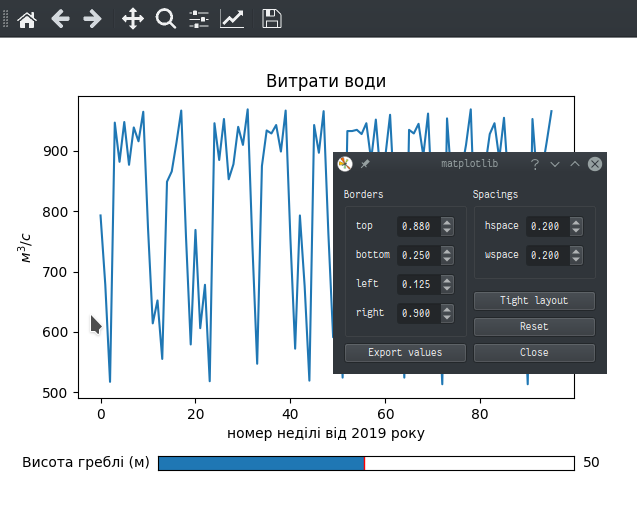
\includegraphics[width=0.7\linewidth]{02.PNG}
	\caption{Приклад інтерфейсу вікна програми.}\label{img:interface}
\end{figure}

На рисунку \ref{img:interface} ми бачимо графік з панеллю для інтерактивної взаємодії з графіком та вікно для налаштування параметрів відображення. За допомогою цього інтерфейсу ми можемо змінювати масштаб графіку, переміщуватися по значенням графіку, та відновлювати початковий стан відображення та можно задати перепад висоти, утворений греблею. Також є можливість експортування значень із графіку. 

У програмі задані такі константи та змінні:
\begin{itemize}
\item $H_{AB}$ - перепад висот, утвореної за допомогою греблі, у ДніпроГЕС це значення дорівнює $50$
\item $T$ - неділя у секундах, має значення $604800$,
\item $g$ - прискорення вільного падіння, має значення $9.8$,
\item $N$ - кількість розглянутих неділь, має значення $96$, що позначає 2 роки.
\item $Q$ - масив показників витрат води у кожну неділю.
\end{itemize}

Задавши ці параметри, програмне забезпечення дозволяє обчислити:

\begin{itemize}
\item $E(t)$ - кількість енергії, яка може бути вироблена за допомогою гідроелектростанції у момент часу $t$,
\item $P(t)$ - швидкість зміни кількості виробляємої енергії, тобто $P(t)=E'(t)$,
\end{itemize}

За замовчанням початкові значення енергії дорівнюють 0.

\newpage

\section{Аналіз отриманих результатів}

Проаналізуємо результати роботи програми для наступних заданих значень параметрів системи та початкових умов:
\begin{itemize}
\item Висоту перепаду води, утвореною за допомогою греблі, встановимо 50 м, та розглянемо також випадок коли висота перепаду буде 25 м.
\item Також встановимо прискорення вільного падіння $g=98.1$ м/с$^2$.
\item Обчислимо та задамо кількість секунд у неділі $60\cdot60\cdot24\cdot7=604800$ с.
\item Також задамо кількість неділь, для яких проводиться аналіз. Було узято 2 роки, що дорівнює 96 неділям.
\item Та задамо показники витрат води за 2019-2020 роки.
\end{itemize}

\begin{figure}[!htb]
	\centering
	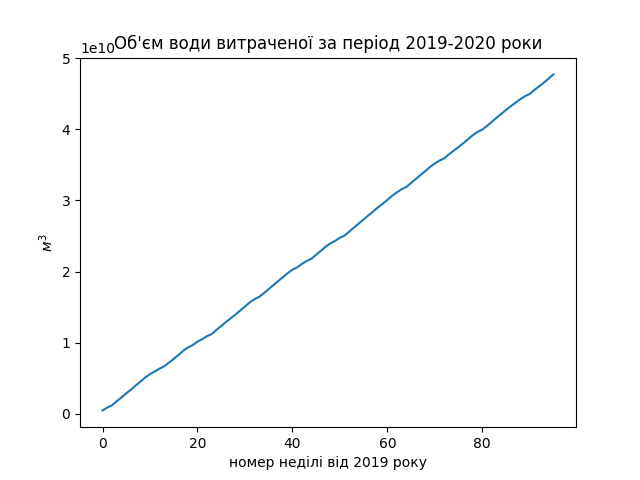
\includegraphics[width=0.7\linewidth]{Figure_1.png}
	\caption{Об'єм води витраченої за період 2019-2020 роки}\label{fig:1}
\end{figure}
\begin{figure}[!htb]
	\centering
	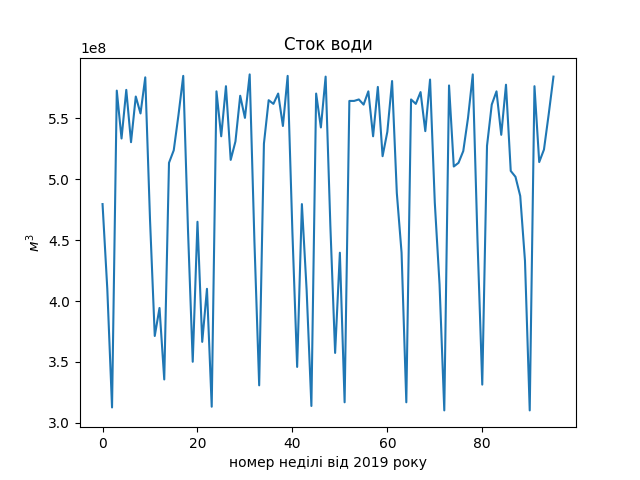
\includegraphics[width=0.7\linewidth]{Figure_6.png}
	\caption{Об'єми води витраченої за кожну неділю}\label{fig:6}
\end{figure}
\begin{figure}[!htb]
	\centering
	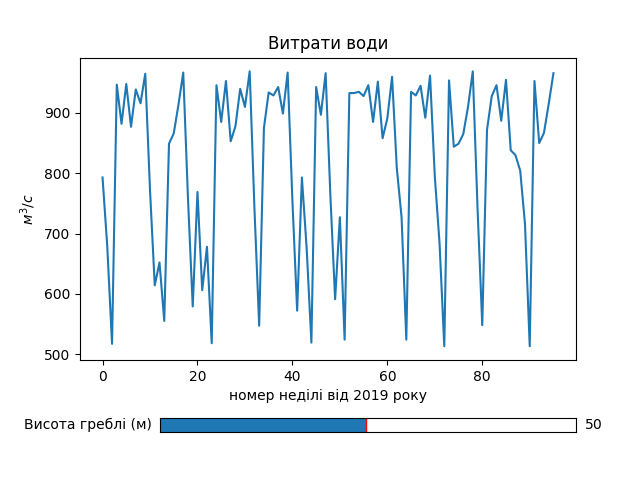
\includegraphics[width=0.7\linewidth]{Figure_2.png}
	\caption{Витрати води}\label{fig:2}
\end{figure}

На рисунках \ref{fig:1}, \ref{fig:6}, \ref{fig:2} ми бачимо вхідні дані витрат води та обчислені об'єми води витраченої за кожну неділю, а також загальні об'єми води витраченої води. Отримали результати: графіки виробництва енергії побудовані відносно всього періоду, потижнево, помісячно.
\newpage

\begin{figure}[!htb]
	\centering
	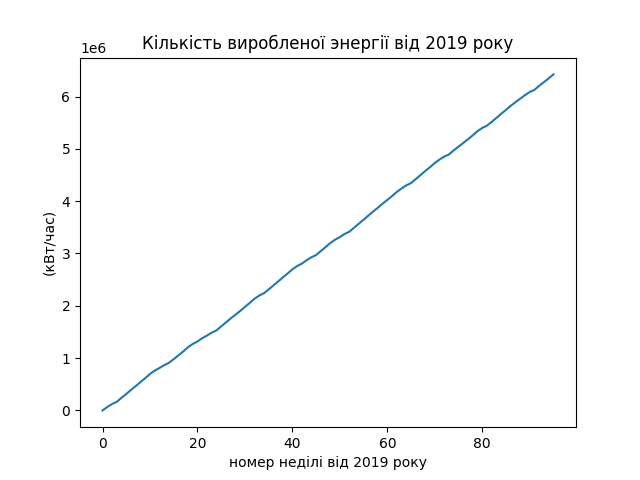
\includegraphics[width=0.7\linewidth]{Figure_3.png}
	\caption{Кількість виробленої енергії від 2019 року, висота перепаду 50 м}\label{fig:3}
\end{figure}
\begin{figure}[!htb]
	\centering
	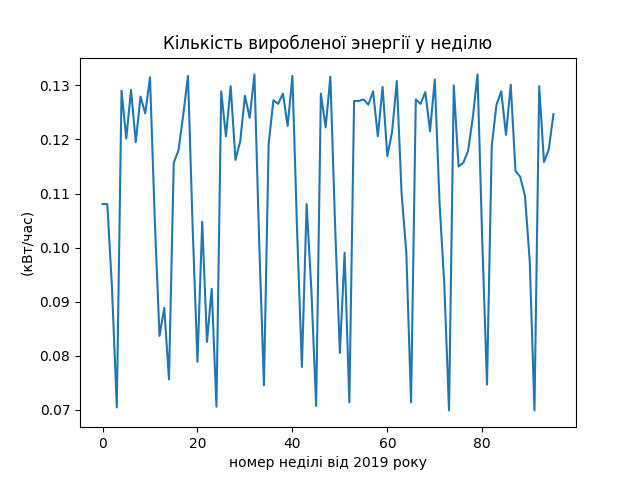
\includegraphics[width=0.7\linewidth]{Figure_4.png}
	\caption{Кількість виробленої енергії у неділю, висота перепаду 50 м}\label{fig:4}
\end{figure}
\begin{figure}[!htb]
	\centering
	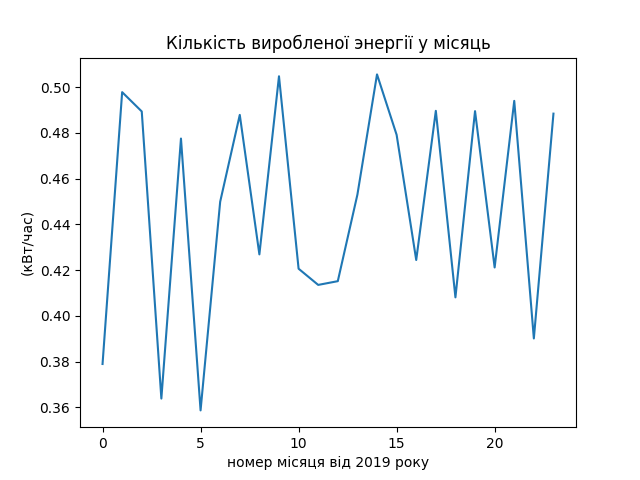
\includegraphics[width=0.7\linewidth]{Figure_5.png}
	\caption{Кількість виробленої енергії у місяць, висота перепаду 50 м}\label{fig:5}
\end{figure}
\begin{figure}[!htb]
	\centering
	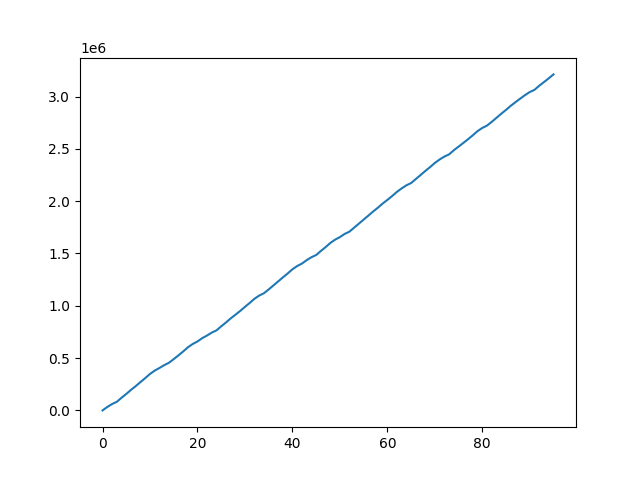
\includegraphics[width=0.7\linewidth]{Figure_25_3.png}
	\caption{Кількість виробленої енергії від 2019 року, висота перепаду 25 м}\label{fig:25_3}
\end{figure}
\begin{figure}[!htb]
	\centering
	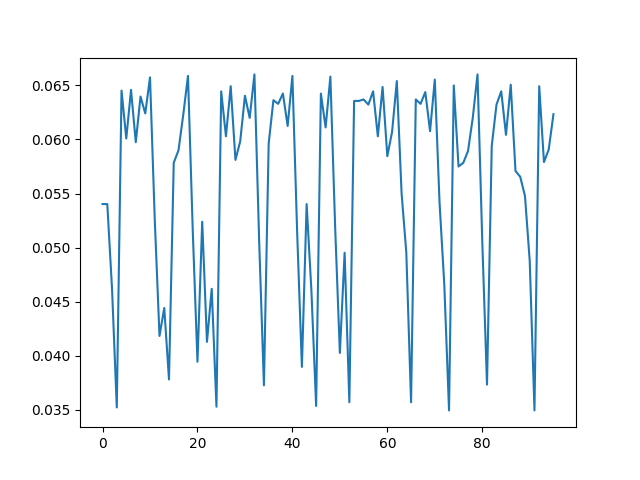
\includegraphics[width=0.7\linewidth]{Figure_25_4.png}
	\caption{Кількість виробленої енергії у неділю, висота перепаду 25 м}\label{fig:25_4}
\end{figure}
\begin{figure}[!htb]
	\centering
	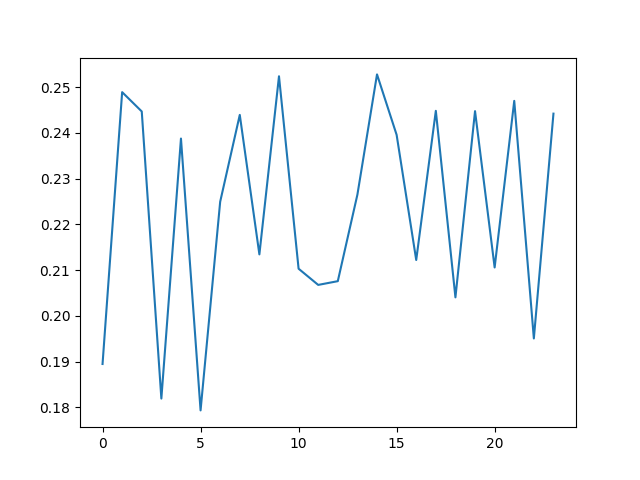
\includegraphics[width=0.7\linewidth]{Figure_25_5.png}
	\caption{Кількість виробленої енергії від 2019 року, висота перепаду 25 м}\label{fig:25_5}
\end{figure}

На рисунках \ref{fig:3}, \ref{fig:4}, \ref{fig:5} бачимо кількості виробленої енергії при висоті перепаду 50 м, та на рисунках \ref{fig:25_3}, \ref{fig:25_4}, \ref{fig:25_5} бачимо кількості виробленої енергії при висоті перепаду 25 м. З цих рисунків можна зробити висновок, що кількість енергії прямо пропорційна витратам води. Також бачимо що залежність від висоти перепаду лінійна. Результати цих досліджень можна використовувати для прогнозу, яке буде виробництво енергії, якщо з плином часу зміниться висота перепаду води.

\section{Висновки}

У ході лабораторної роботи було:
\begin{enumerate}
\item Проведено огляд джерел предметної області та розглянути існуючі підходи до побудови математично моделі гідроелектростанції.

\item Побудувано математичну модель гідроелектростанції ДніпроГЕС, використовуючи підхід на основі балансових співвідношень. Для наближеного розв'язку задачу Коші було використано метод Ейлера.

\item Розроблене програмне забезпечення на мові Python на основі побудованої математичної моделі та знайдено наближений розв'язок задачі методом Ейлера.

\item Проведено дослідження отриманого розв'язку математичної моделі ДніпроГЕС при різних значеннях параметрів системи.
\end{enumerate}

\newpage

\section{Перелік використаних джерел}

\begin{enumerate}
\item Пантелеев В.И. Многоцелевая оптимизация и автоматизированное проектирование управления качеством электроснабжения в электроэнергетических системах: монография/ В.И. Пантелеев, Л.Ф. Поддубных. – Красноярск :Изд-во Сиб. федер. ун-т, 2009. – 194 с.
\item Борщ П.С. Методика планирования выработки электроэнергии каскада ГЭС с учетом стокообразующих и атмосферных факторов : дис. ... канд. техн.наук :05.14.08 / Борщ Павел Сергеевич. – Москва, 2014. –147 с.
\item Ильиных И. И. Гидроэлектростанци: Учебник для техникумов. // М.: Энергоатомниздат. - 1988. - 2-ое изд. - 248 с.
\item Крючковский В.В. Ситуационный подход к теории организации и управления промышленными объектами в условиях неопределенности /В.В. Крючковский, И.Ф.Погребняк, А.В. Шарко // Экономичные инновации. –2011. – Вып. 45. – С. 132–137.
\item Глазунова А.М. Модифицированное оценивание состояния для решения диспетчерских задач при управлении режимами электроэнергетической системы / А.М.Глазунова, Е.С. Аксаева // Электричество. – 2013. – No 12. –С. 21–29.
\item ПрАТ Укргідроенерго - Основні показники -- 2021 -- Режим доступу:  

https://uhe.gov.ua/diyalnist/osnovni\_pokaznyky
\end{enumerate}

\section{Лістинг програми}

\begin{pythoncode}
#!/usr/bin/env python3

import numpy as np
import matplotlib.pyplot as plt
from datetime import tzinfo, timedelta, date

N = 96
h = 60*60*24*7
g = 9.81
H = 50

weeks = np.arange(0, N, 1)
y = np.array([793, 678, 517, 947, 882, 948, 877, 939, 916, 965, 772, 614, 652, 555, 849, 866, 914, 967, 758, 579, 769, 606, 678, 518, 946, 885, 953, 853, 878, 940, 910, 969, 742, 547, 875, 934, 929, 943, 899, 967, 755, 572, 793, 676, 519, 943, 897, 966, 763, 591, 727, 524, 933, 933, 935, 928, 946, 885, 952, 858, 891, 960, 808, 727, 524, 935, 929, 945, 892, 962, 795, 684, 513, 954, 844, 849, 865, 910, 969, 743, 548, 872, 928, 946, 887, 955, 838, 830, 804, 716, 513, 953, 850, 867, 915, 966])

start_date = date(2019, 1, 1)
dweek = timedelta(weeks=1)

for i in range(32):
    print("%s & %s & %s & %s & %s & %s \\\\\\hline"
        % ((start_date+dweek*i).isoformat(), y[i], (start_date+dweek*(i+32)).isoformat(), y[i],
           (start_date+dweek*(i+64)).isoformat(), y[i]))


volume_per_week = lambda H: y*h
volume = lambda H: np.add.accumulate(volume_per_week(H))

def e(H):
    e = np.zeros(N)
    for i in range(N-1):
        e[i+1] = e[i] + h * g * y[i] * H
    return e/1000/3600

def de(H):
    de = np.zeros(N)
    de[0] = g * y[0] * H

    for i in range(N-1):
        de[i+1] = g * y[i] * H
        
    return de/1000/3600
    
def dem(H):
    dev = de(H)
    return np.array([sum(dev[4*i:4*i+4]) for i in range(N//4)])

fig1 = plt.figure(1)
ax1 = fig1.add_subplot(1,1,1)
p1, = ax1.plot(weeks, volume(H))
plt.title('Об\'єм води витраченої за період 2019-2020 роки')
plt.xlabel('номер неділі від 2019 року')
plt.ylabel('$м^3$')

fig6 = plt.figure(6)
ax6 = fig6.add_subplot(1,1,1)
p6, = ax6.plot(weeks, volume_per_week(H))
plt.title('Сток води')
plt.xlabel('номер неділі від 2019 року')
plt.ylabel('$м^3$')

fig2 = plt.figure(2)
ax2 = fig2.add_subplot(1,1,1)
p2, = ax2.plot(weeks, y)
plt.title('Витрати води')
plt.xlabel('номер неділі від 2019 року')
plt.ylabel('$м^3/c$')

plt.subplots_adjust(bottom=0.25)

axfreq = plt.axes([0.25, 0.1, 0.65, 0.03])
height_slider = plt.Slider(
    ax=axfreq,
    label='Висота греблі (м)',
    valmin=1,
    valmax=100,
    valstep=1,
    valinit=H,
)

fig3 = plt.figure(3)
ax3 = fig3.add_subplot(1,1,1)
p3, = ax3.plot(weeks, e(H))
plt.title('Кількість виробленої энергії від 2019 року')
plt.xlabel('номер неділі від 2019 року')
plt.ylabel('(кВт/час)')

fig4 = plt.figure(4)
ax4 = fig4.add_subplot(1,1,1)
p4, = ax4.plot(weeks, de(H))
plt.title('Кількість виробленої энергії у неділю')
plt.xlabel('номер неділі від 2019 року')
plt.ylabel('(кВт/час)')

fig5 = plt.figure(5)
ax5 = fig5.add_subplot(1,1,1)
p5, = ax5.plot(range(N//4), dem(H))
plt.title('Кількість виробленої энергії у місяць')
plt.xlabel('номер місяця від 2019 року')
plt.ylabel('(кВт/час)')


def update(val):
    H = height_slider.val
    ax1.clear()
    p1, = ax1.plot(weeks, volume(H))
    fig1.canvas.draw_idle()
    ax3.clear()
    p3, = ax3.plot(weeks, e(H))
    fig3.canvas.draw_idle()
    ax4.clear()
    p4, = ax4.plot(weeks, de(H))
    fig4.canvas.draw_idle()
    ax5.clear()
    p5, = ax5.plot(range(N//4), dem(H))
    fig5.canvas.draw_idle()


height_slider.on_changed(update)

plt.show()
\end{pythoncode}

\end{document}